\section{IP (Network Layer)}

\subsection{Router/Gateway}
Verbinden verschiedene Netze mit potentiell unterschiedlichen Technologien

Lösen 2 Aufgaben:
\begin{description}
    \item[Routing] Aufbau und Update von Routingtabellen
    \item[Forwarding] Weiterleiten der Pakete anhand Routingtabellen
\end{description}

\subsubsection{Routing-Tabelle}
löst: wie Kann ich welches Netz erreichen?

Bei hierarchischem Routing (Router wissen welche Netze an anderen Router sind
forwarden entsprechend) kommen oft auch aggregierte Routen vor.\\
Wenn so z.B. 130.0.0.0/25 und 130.0.128.0/25 beide via den selben Router
erreichbar sind wird diese Route aggregiert und als 130.0.0.0/24 zusammengefasst.

\begin{center}
    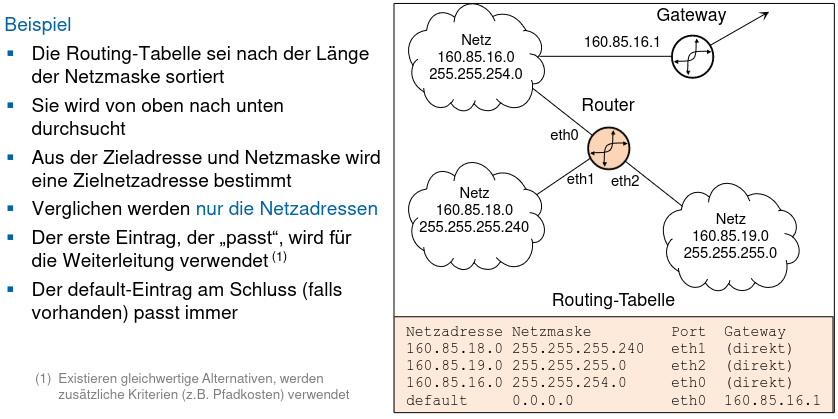
\includegraphics[width=0.9\linewidth]{routing-table}
\end{center}

\subsubsection{Classful Routing}

Ursprünglich wurden IP Adressen in 5 Routing Klassen eingetelt (Classful Routing).
Die ersten vier Adressbits erlauben eine Bestimmung der Klasse.
Wird nicht mehr gemacht weil oftmals Adressraum verschwendet wird.

\begin{center}
    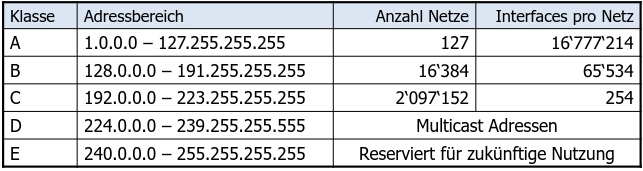
\includegraphics[width=0.9\linewidth, height=15mm]{classful-routing}
\end{center}

\subsubsection{Subnetting}
\begin{itemize}
    \item das Netz in kleinere Subnetze teilen
    \item funktioniert simplifiziert durch beliebiges erweitern der Netzadresse
    \item hintereinanderliegende Netze können zusammengefügt werden
          \begin{center}
              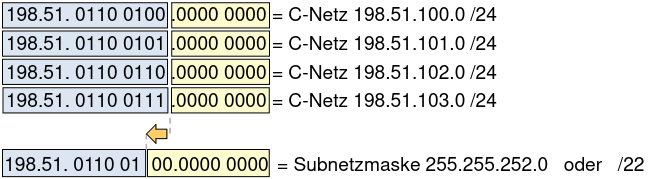
\includegraphics[width=0.8\linewidth, height=10mm]{subnetting-aggr}
          \end{center}
          % \begin{itemize}
          %  \item 160.85.100.0/24
          %  \item 160.85.101.0/24
          %  \item 160.85.102.0/24
          %  \item 160.85.103.0/24
          %  \item zusammengefügt: 160.85.100/22
          % \end{itemize}
\end{itemize}








\subsection{Adressierung / IPv4}

Adresse eines Host = Netz-Adresse + Interface-Adresse

\subsubsection{Subnetzmaske}

\begin{center}
    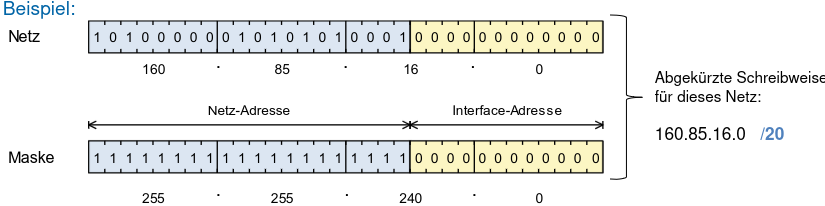
\includegraphics[width=0.9\linewidth]{subnetmask}
\end{center}

\subsubsection{Netzadresse}

\begin{itemize}
    \item reserviert, darf NICHT für interfaces verwendet werden
    \item tiefste Adresse im Subnet $\rightarrow$ alle interface bits 0
    \item berechnung durch $Interface Adresse \land Subnetzmaske$
\end{itemize}

\subsubsection{Broadcast-Adresse}

\begin{itemize}
    \item reserviert, darf NICHT für interfaces verwendet werden
    \item höchste Adresse im Subnet $\rightarrow$ alle interface bits 1
    \item berechnung durch $Interface Adresse \lor invertierte \, Subnetzmaske$
\end{itemize}

\subsubsection{Private Adressen}

Die $172.0.0.0/8$ Adressen sind reserviert für Loopback und verlassen den Host nicht.
Sie werden an ein emuliertes Loopback-Gerät geschickt dass direkt returned
(kein Interface nötig).
\begin{center}
    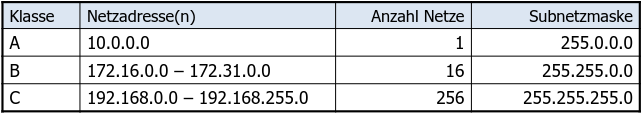
\includegraphics[width=0.9\linewidth, height=10mm]{private-ip}
\end{center}



\subsection{IPv4 Header}

\textcolor{red}{immer minimum 4Byte Blöcke}

\begin{center}
    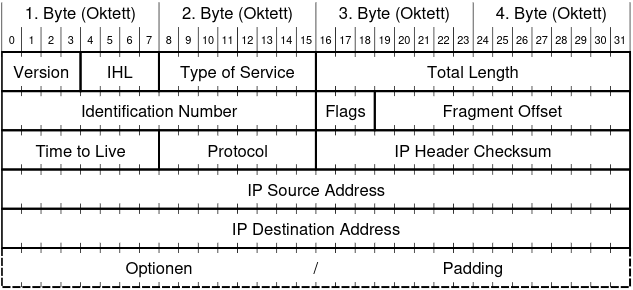
\includegraphics[width=0.9\linewidth]{ip4-header}
\end{center}

\begin{description}
    \item[Version] 4 oder 6
    \item[IHL] Internet Header Length ( / 4 weil immer 4 Byte Blöcke)
        \begin{itemize}
            \item Header ohne optionen = 20 Bytes $\rightarrow$ IHL = 5
            \item Maximalwert 15 (4 Bits)
        \end{itemize}
    \item[TOS] Type of Service, erlaubt prioriesierung
        \begin{center}
            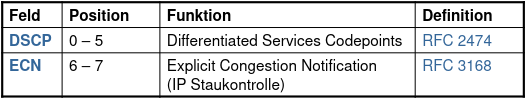
\includegraphics[width=0.9\linewidth, height=10mm]{ip4-tos}
        \end{center}
    \item[Total Length] inclusive Header \& Nutzdaten
    \item[TTL] Time To Live, In Anzahl Hops. Verhindern Loops, jeder Router
        dekrementiert, bei 0 $\rightarrow$ Paket verwerfen
    \item[Protocol] Protokoll der Nutzdaten
        \begin{enumerate}
            \item[1] ICMP Internet Control Message Protocol
            \item[6] TCP Transport Control Protocol
            \item[17] UDP User Datagramm Protocol
        \end{enumerate}
    \item[Header Checksum] schütz NUR den Header, bei jedem Router neu berechnet(TTL)
    \item[Options/Padding] variabel, heute selten, Padding für 32 bits
    \item[Identification Number] identifikation, bleibt für fragmentierte Pakete gleich
    \item[Flags] 3 Bits, steuert Fragmentierung über einzelne Bits
        (Aufzählung von links aus)
        \begin{enumerate}[start=0]
            \item reserviert, immer 0
            \item DF, 0/1 $\rightarrow$ May / Dont Fragment
            \item MF, 0/1 $\rightarrow$ Last / More Fragments
        \end{enumerate}
    \item[Fragment Offset] 13 Bits, steht für Anzahl 8 Byte Blöcke, bestimmt
        wo im gesamt paket die Daten hingehören
\end{description}


\subsubsection{Fragmentierung}

IP-Paket maximal 65535 Bytes, aber limitiert durch MTU des Netz. \\
Problem: spätere Netze haben eventuell tiefere MTU $\rightarrow$ Fragmentierung.

\begin{itemize}
    \item jedes Fragment erhält seinen eigenen Header
    \item Identification Number bleibt gleich
    \item Total Length jeweils die Länge des Paket
    \item alle Pakete ausser letztes haben MF = 1 in den Flags
    \item alle Pakete haben die gleiche, vielfaches von 8, maximale Länge (ausser letzes)
\end{itemize}
\begin{center}
    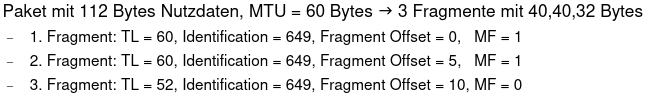
\includegraphics[width=0.9\linewidth, height=10mm]{ip4-fragment-ex}
\end{center}


\subsubsection{Reassembly}

\begin{itemize}
    \item Fragmente werden erst beim Zielhost zusammengesetzt
    \item Pakete mit FO = MF = 0 sind ''komplett'' $\rightarrow$ brauchen kein Reassembly
    \item für alle anderen (=Fragmente) wird folgende Datenstruktor alloziert
          \begin{enumerate}
              \item Daten-Buffer für grösstmögliches Paket (64KB)
              \item Header-Buffer zur Rekonstruktion des original Headers
              \item Timer (ca. 15 Sekunden Timeout)
          \end{enumerate}
\end{itemize}

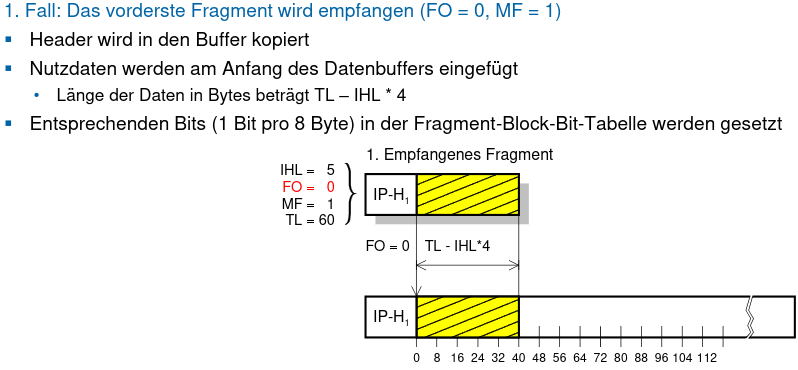
\includegraphics[width=0.9\linewidth, height=23mm]{ip-reassembly-case-first}

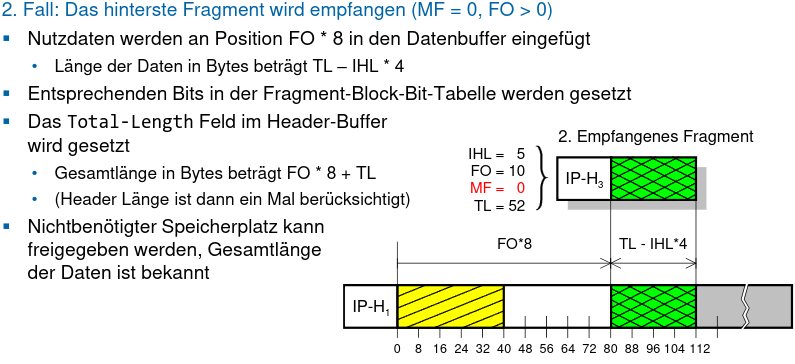
\includegraphics[width=0.9\linewidth, height=23mm]{ip-reassembly-case-last}

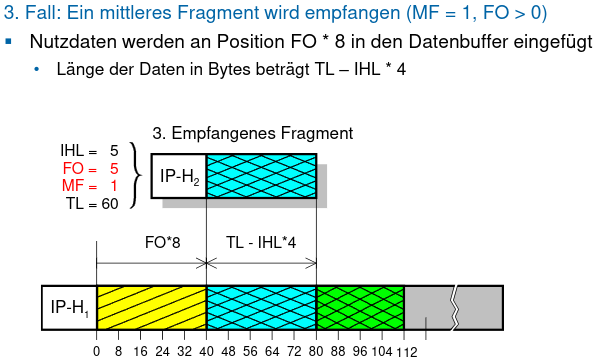
\includegraphics[width=0.7\linewidth, height=21mm]{ip-reassembly-case-between}




\subsection{Kapselung}

\begin{itemize}
    \item Ethernet-Encapsulation: das IP-Paket wird als Data des Ethernet Frame übertragen $\rightarrow$ MTU = 1500
    \item Type im Ethernet-Frame = 0x0800
\end{itemize}

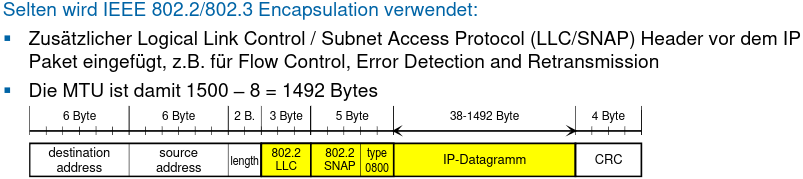
\includegraphics[width=0.9\linewidth, height=15mm]{ip4-802-3-encap}

\subsubsection{Übertragung mit Encapsulation}

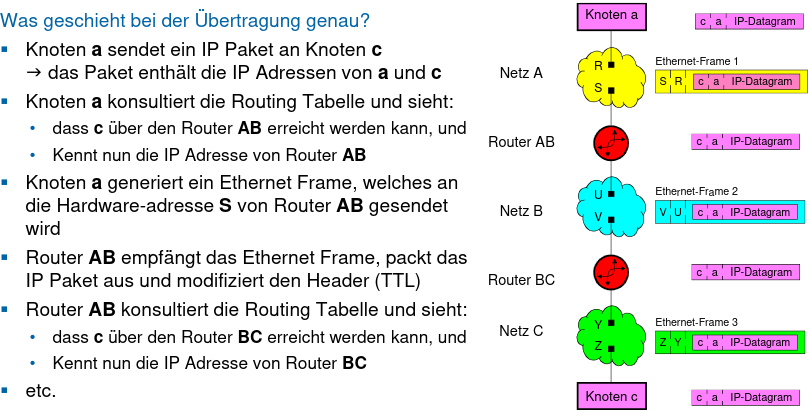
\includegraphics[width=0.9\linewidth, height=27mm]{ip4-encap-transmission}




\subsection{Adressauflösung mit Address Resolution Protocol (ARP)}

\begin{itemize}
    \item NICHT teil von IP selbst
    \item Löst: Host a möchte die Hardware Adresse für die IP Adresse 160.85.20.33
    \item jeder Host führt lokalen ARP-Cache für bekannte Adressen
    \item commands:
          \begin{itemize}
              \item arp -a / ip neigh show
              \item arp -d <ipaddr> / ip neigh del
              \item arp -s <ipaddr> <hwaddr> / ip neigh add
          \end{itemize}
    \item Gratuitous ARP (unnötig/unbegründet)
          \begin{itemize}
              \item z.B. von Windows nach dem Starten
              \item nach Adresszuweisung wird ARP request an eigene IP gesendet
                    für Konflikterkennung
              \item gratuitous reply für e.g. Cache-Refresh / Broadcast
          \end{itemize}
\end{itemize}

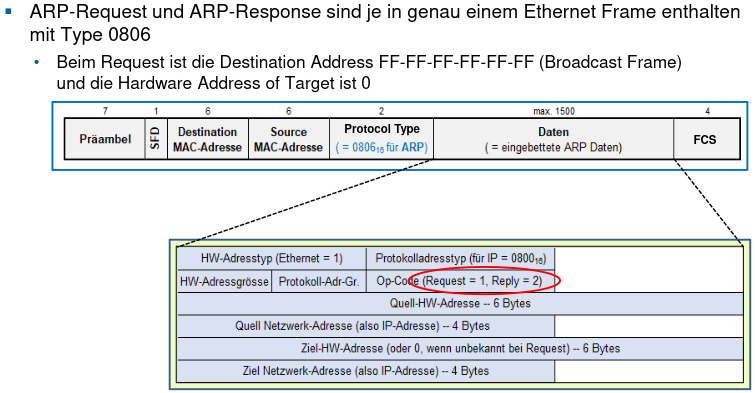
\includegraphics[width=0.9\linewidth, height=27mm]{arp-struct}



\subsection{Internet Control Message Protocol ICMP}

\begin{itemize}
    \item Fehlermeldungen auf Internet Layer (TTL = 0)
    \item Test ob anderer Host erreichbar ist (ping)
    \item Gekaplelt in IP Paketen aber wird zu Network Layer gezählt
    \item gebräuchliche Typen (in ICMP header)
          \begin{description}
              \item \textcolor{red}{Fehler:}
              \item[3] Destination Unreachable - e.g. Dont Fragment gesetzt aber
                  MTU zu klein
              \item[5] Redirect - Router merkt dass Host direkteren Weg nehmen könnte
                  $\rightarrow$ Host sendet vervolständigt Routingtabelle und nimmt
                  direkten weg
              \item[11] Time Exceeded -  Router setzt TTL = 0 oder Timeout für Fragmente
              \item[12] Parameter Problem: Bad IP Header - IP Header hat ungültigen
                  Wert
              \item \textcolor{blue}{Information:}
              \item[0] Echo Reply - Host erhält Echo Request
                  $\rightarrow$ Echo Reply mit gleichen Daten
              \item[8] Echo (Request) - Host sendet Echo Request (ping)
              \item[13] Timestamp - Wie Echo aber mit Timestamp austausch
              \item[14] Timestamp Reply
          \end{description}
\end{itemize}

\subsubsection{ICMP Echo / Reply}

\begin{center}
    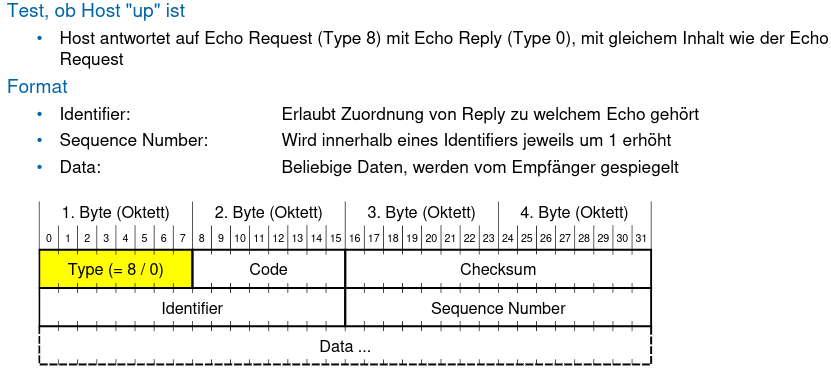
\includegraphics[width=0.9\linewidth, height=23mm]{icmp-echo-reply}
\end{center}


\subsubsection{ICMP Destination Unreachable}

\begin{center}
    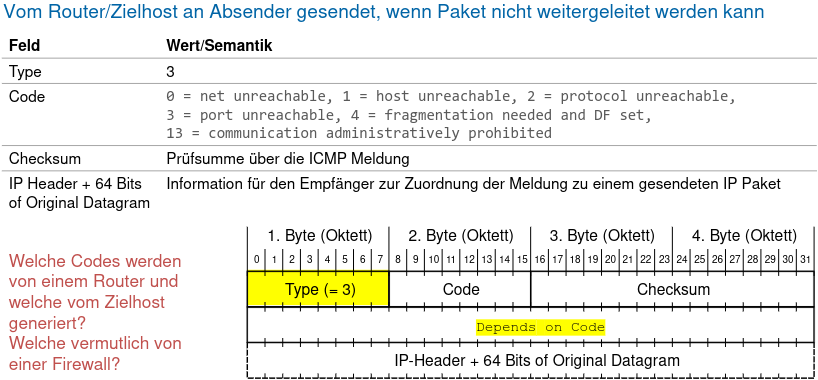
\includegraphics[width=0.9\linewidth, height=23mm]{icmp-dest-unreach}
\end{center}

\subsubsection{ICMP Time Exceeded}

Wird auch für \textcolor{blue}{traceroute} verwendet, durch inkrementelles erhöhen der TTL
können die IP-Adressen der zwischen liegenden Router aus den ICMP Fehlern
herausgefunden werden.

Linux command beispiel: \lstinline[language=sh]{traceroute -n -q1 <ip-addr>}

\begin{center}
    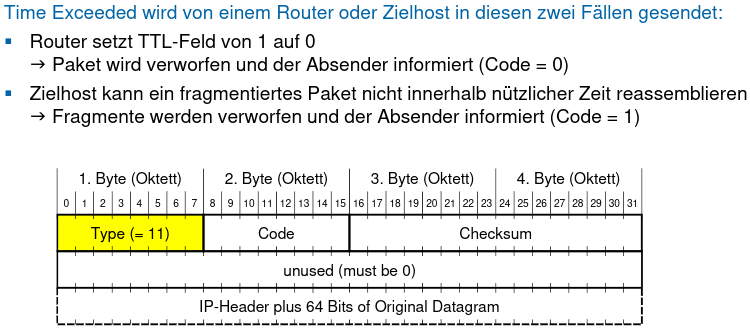
\includegraphics[width=0.9\linewidth, height=23mm]{icmp-time-exceeded}
\end{center}
